\documentclass[11pt]{article}
\usepackage[left=1in,top=1in,right=1in,bottom=1in,head=.1in,nofoot]{geometry}

\setlength{\footskip}{24pt} % Page number/footer spacing
\usepackage{setspace,url,bm,amsmath} % For double-spacing, URL font, math symbols

\usepackage{titlesec} % Section header formatting
\titlelabel{\thetitle.\quad} % Section header formatting
%\titleformat*{\section}{\bf\large\center\uppercase} % Section header formatting

\usepackage{graphicx} % Graphics scaling
\usepackage{bbm, amssymb}
\usepackage{latexsym}
\usepackage{caption}
\usepackage[margin=20pt]{subcaption}
\usepackage{hyperref, enumerate}
\usepackage[all,import]{xy}




\usepackage[table]{xcolor}
%\newcommand\x{\times}
%\newcommand\y{\cellcolor{green!10}}
\newcommand\y[1]{%
  \colorbox{green!10}{$#1$}%
}
\newcommand{\GG}[1]{}

\usepackage{amsthm}
%\usepackage{undertilde}
\usepackage{comment}
\theoremstyle{definition}
\newtheorem{assumption}{Assumption}
\newtheorem*{theorem*}{Theorem}
\newtheorem{theorem}{Theorem}
\newtheorem{proposition}{Proposition}
\newtheorem{lemma}{Lemma}
\newtheorem{remark}{Remark}
\newtheorem{exercise}{Exercise}
\newtheorem{example}{Example}
\newtheorem{excont}{Example}
\renewcommand{\theexcont}{\theexample}

\newtheorem{definition}{Definition}
\newtheorem{corollary}{Corollary}
\newtheorem*{corollary*}{Corollary}




\usepackage{natbib} % ASA citation style
\bibpunct{(}{)}{;}{a}{}{,} % ASA citation style

\renewcommand{\refname}{REFERENCES} % Capitalize bibliography section header
\usepackage{etoolbox} % Bibliography underfull/overfull box fix
\apptocmd{\sloppy}{\hbadness 10000\relax}{}{} % Bibliography underfull/overfull box fix

\usepackage{color}
\usepackage{listings}


\DeclareMathOperator*{\Med}{Med}
\DeclareMathOperator*{\argmin}{arg\,min}
\DeclareMathOperator*{\argmax}{arg\,max}


\newcommand{\pkg}[1]{{\fontseries{b}\selectfont #1}}
\def\letas{\mathrel{\mathop{=}\limits^{\triangle}}}
\def\ind{\begin{picture}(9,8)
         \put(0,0){\line(1,0){9}}
         \put(3,0){\line(0,1){8}}
         \put(6,0){\line(0,1){8}}
         \end{picture}
        }
\def\nind{\begin{picture}(9,8)
         \put(0,0){\line(1,0){9}}
         \put(3,0){\line(0,1){8}}
         \put(6,0){\line(0,1){8}}
         \put(1,0){{\it /}}
         \end{picture}
    }

\def\AVar{\text{AsyVar}}
\def\Var{\text{var}}
\def\var{\text{var}}
\def\Cov{\text{cov}}
\def\cov{\text{cov}}
\def\sumn{\sum_{i=1}^n}
\def\summ{\sum_{j=1}^m}
\def\convergeas{\stackrel{a.s.}{\longrightarrow}}
\def\converged{\stackrel{d}{\longrightarrow}}
\def\convergep{\stackrel{p}{\longrightarrow}}
\def\iidsim{\stackrel{i.i.d.}{\sim}}
\def\indsim{\stackrel{ind}{\sim}}
\def\N{\mathcal{N}}
\def\d{\textup{d}}
\def\KL{\textsc{KL}}
\def\obs{\textnormal{obs}}
\newcommand{\pr}{\textnormal{pr}}
\def\FRT{\text{Fisher randomization test}}
\def\asim{\stackrel{\cdot}{\sim}}
\def\DCE{\textsc{DCE}}

\begin{document}
\doublespacing
\title{\bf  Problem Set 2\\
Due October 7th, 6:40 pm
}
\date{}
\maketitle


\section{Neymanian inference and OLS}


Consider a completely randomized experiment with $n$ units. For unit $i$, let $Z_i$ be the binary treatment indicator and $Y_i$ be the observed outcome. We have discussed the Neymanian inference for the average causal effect in class, i.e, the unbiased estimator $\hat{\tau}$ and a conservative estimator for its variance $\hat{V}$. 

Practitioners often use regression-based inference for the average causal effect, i.e., running OLS of the outcomes on the treatment indicators and using the coefficient of the treatment as the estimator. Show that
\begin{enumerate}
[(1)]
\item
this point estimator is identical to Neyman's unbiased estimator $\hat{\tau}$;

\item
the variance estimator from the classical OLS (for example, the one reported by the lm function of R) can be asymptotically different from $\hat{V}$, i.e., their ratio does not converge to 1 in probability even with a large sample size;

\item
the Eicker--Huber--White variance estimator from the OLS is asymptotically equivalent to $\hat{V}$, i.e., their ratio converges to 1 in probability. 
Note that if you run OLS of $Y_i$ on $W_i = (1,Z_i)$ with coefficient $\hat{\beta}$, the Eicker--Huber--White variance estimator for the coefficient is
$$
(W'W)^{-1} W' \text{diag}( \hat{e}_1^2, \ldots, \hat{e}_n^2 ) W (W'W)^{-1},
$$
where $W$ is the matrix with rows of $(1,Z_i)$ and $\hat{e}_i = Y_i  - W_i \hat{\beta}$ is the residual from the OLS. 
\end{enumerate}





\section{FRT for the Project STAR data in the Imbens--Rubin book}

Reanalyze the Project STAR data in Table 9.1 (at the end of this file) using the Fisher randomization test. Note that I use $Z$ for the treatment indicator but the book uses $W.$ Use $\hat{\tau}_\textsc{S}$, $V$ and the aligned rank statistic in the  Fisher randomization test. Compare the $p$-values.










\section{Data re-analyses}

\begin{enumerate}
[(1)]
\item
Re-analyze the LaLonde data used in \texttt{Neymanlalonde.R}. Conduct both Fisherian and Neymanian inferences. 

The original experiment is a completely randomized experiment. Now we pretend that the original experiment is a stratified randomized experiment.
First, re-analyze the data pretending that the experiment is stratified on the race (black, Hispanic or other). Second, re-analyze the data pretending that the experiment is stratified on marital status. Third, re-analyze the data pretending that the experiment is stratified on the indicator of high school diploma. 

Compare with the results obtained under a completely randomized experiments. 

\item
Re-analyze the data used in \texttt{SRE\_Neyman\_penn.R}. The analysis in class uses the treatment indicator, the outcome and the block indicator. Now we want to use all other covariates. 

Conduct regression adjustments within strata of the experiment, and then combine these adjusted estimators to estimate the average causal effect. Report the point estimator, estimated standard error and 95\% confidence interval. Compare them with those without regression adjustments. 


\end{enumerate}


\section{Regression adjustment / post-stratification of CRE}


In a completely randomized experiment, we have a binary treatment indicator $Z$, an outcome $Y$, and a discrete covariate $X \in \{  1, \ldots, K \}$. We can use two methods to use covariates to improve estimation efficiency. 

First, we can use the post-stratification estimator, pretending that the experiment is a stratified randomized experiment, conditional on $X$. This estimator is $\hat{\tau}_{\textsc{ps}}$. 

Second, we can create $K-1$ dummy variables $\delta_{1i} = I(X_i=1), \ldots, \delta_{K-1,i} = I(X_i=K-1)$, and use Lin's estimator with covariates $\delta_1,\ldots, \delta_{K-1}$. This estimator is $\hat{\tau}_\textsc{L}$. 

Show that $\hat{\tau}_{\textsc{ps}} = \hat{\tau}_\textsc{L}.$ Note that sometimes $\hat{\tau}_{\textsc{ps}}$ or $ \hat{\tau}_\textsc{L}$ may not be well-defined. In those cases, we treat $\hat{\tau}_{\textsc{ps}}$ and $ \hat{\tau}_\textsc{L}$ as equal. 


For students in Stat 157, you can assume that $K=2$.


\section{Additional comments on the Neymanian inference under an SRE (Problem (2) only for Stat 260)}


\begin{enumerate}
[(1)]
\item
Show that if $e_{[k]} = e$ for all $k$, then $\hat{\tau} = \hat{\tau}_\textsc{S}.$

\item 
Assume that the individual causal effect is constant $\tau_i = \tau$ for all $i=1,\ldots, n$. 
Consider the following class of weighted estimator for $\tau$:
$$
\hat{\tau}_w = \sum_{k=1}^K  w_{[k]}  \hat{\tau}_{[k]} ,
$$
where $w_{[k]} \geq 0$ for all $k$.

When will $\hat{\tau}_w $ be unbiased for $\tau$? Among all unbiased estimators, find the one with minimum variance. 


\end{enumerate}


 


\begin{figure}
\centering
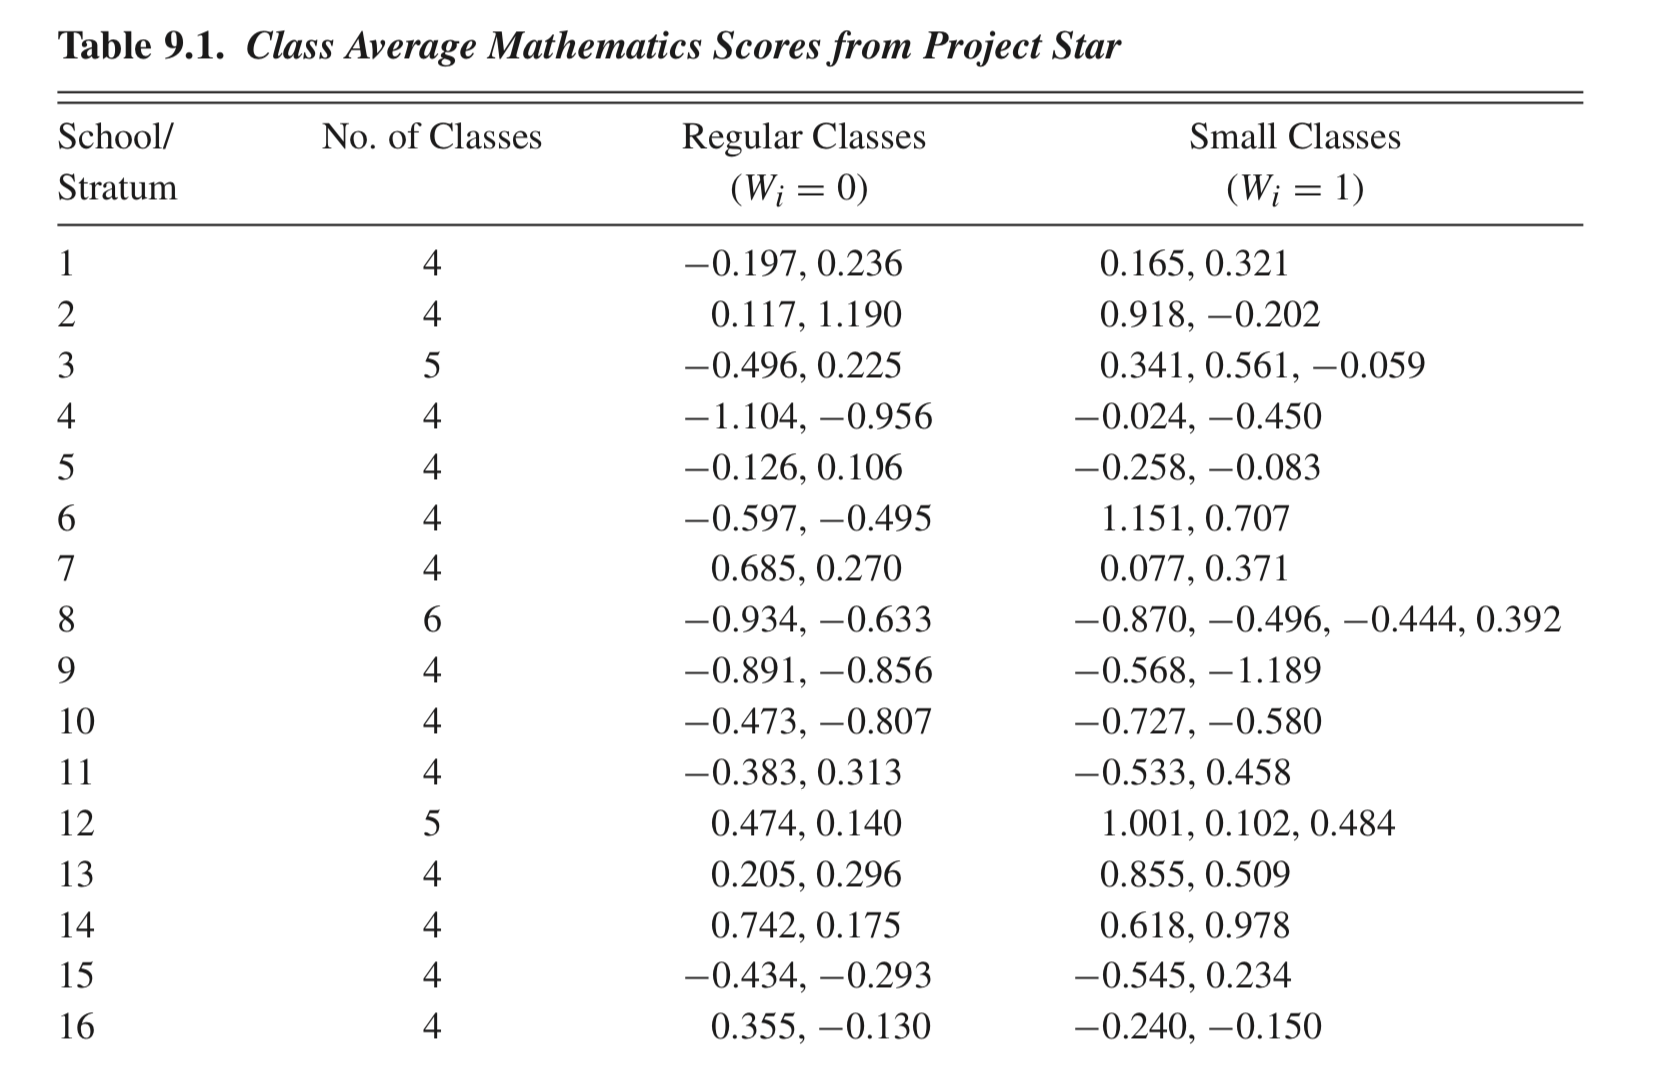
\includegraphics[width = \textwidth]{table9_1.png}
\end{figure}



\bibliographystyle{apalike}
\bibliography{causal}

\end{document}



